%% MAC-IRL — ICAIF '26 submission
%% Template: acmart sigconf + anonymous (required by ICAIF '26 CFP)
%% Compile: pdflatex -> bibtex -> pdflatex -> pdflatex   (or use Overleaf)
%% HARD LIMIT: 8 pages total, including all figures and references.
%% Double-blind: no author names/affiliations; cite own work in third person.
%%
%% STATUS (2026-07-26)
%%   Section 1  : drafted and revised (this file)
%%   Sections 2-5: skeleton only — see docs/paper_ch2_kr.md, docs/paper_ch34_kr_revised.md
%%   Numbers    : canonical run = runs/continuous_reward3_lambda_unified/  (lambda unified at 0.005)
%%   Validation : runs/continuous_reward3_lambda_validation/
%%   References : verified 2026-07-24, see docs/refs_checklist.md
%%   Checklist  : docs/paper_checklist.md

\documentclass[sigconf,anonymous,review]{acmart}

%% Figure 1 (the Section 3 pipeline) is drawn in TikZ so that its symbols
%% are typeset in the body font rather than baked into a bitmap.
\usepackage{tikz}
\usetikzlibrary{arrows.meta,positioning,fit,backgrounds,calc}

\AtBeginDocument{%
  \providecommand\BibTeX{{Bib\TeX}}}

%% Rights: placeholder values until the rights form is completed.
\setcopyright{acmlicensed}
\copyrightyear{2026}
\acmYear{2026}
\acmDOI{XXXXXXX.XXXXXXX}
\acmConference[ICAIF '26]{7th ACM International Conference on AI in
  Finance}{November 14--17, 2026}{Milan, Italy}
\acmISBN{978-1-4503-XXXX-X/2026/11}

\begin{document}

%% The optional argument is the RUNNING HEAD. Without it acmart puts the
%% full title in the header on odd pages, where it collides with the
%% conference line. Added 2026-07-28.
\title[Same Signals, Different Actions]{Same Signals, Different Actions:
  Recovering and Validating
  Investor-Type Preferences from Daily Flow via Inverse Reinforcement
  Learning}

%% NOTE: ICAIF '26 review is DOUBLE-BLIND. The "anonymous" class option
%% suppresses the author block below in the compiled PDF, so the
%% submission stays anonymous while the information is retained here for
%% the camera-ready version. Remove "anonymous" only after acceptance.
\author{Yonghwa Shin}
\affiliation{%
  \institution{Soongsil University}
  \city{Seoul}
  \country{Republic of Korea}}
\email{andysheen607@gmail.com}

\author{Yumin Kwon}
\affiliation{%
  \institution{Soongsil University}
  \city{Seoul}
  \country{Republic of Korea}}

\begin{abstract}
Foreign, institutional, and retail investors trade the same asset for
different reasons, yet the regularities that describe them---momentum
versus contrarian trading, the disposition effect, herding---have been
established one phenomenon at a time, leaving no common scale on which
their preferences can be compared. We build such a scale with inverse
reinforcement learning: each type is an agent whose daily net-buy
intensity reveals a latent reward over three shared market-state features
and two market contexts, and all three types are estimated under a
shared specification, so that differences come only from what is learned.
Under a one-step horizon this estimator coincides with a Lasso; our
contribution is therefore a validation protocol rather than a new
estimator---out-of-sample stability under combinatorial purged
cross-validation, block bootstrap and walk-forward re-estimation,
construct-validity checks against independently established behavioral
regularities, and explicit disclosure of null results. On 973 trading
days of Samsung Electronics (005930) flow, the recovered rewards separate
along the momentum axis: foreign $+0.044$ against retail $-0.036$ in
standardized units, each sign-consistent across all 45 out-of-sample
splits. Institutional flow shows no identified preference despite
converged optimization, and we report this null as a
finding. We make no claim of return predictability.
\end{abstract}

\begin{CCSXML}
<ccs2012>
 <concept>
  <concept_id>10010147.10010257.10010293.10010294</concept_id>
  <concept_desc>Computing methodologies~Inverse reinforcement learning</concept_desc>
  <concept_significance>500</concept_significance>
 </concept>
 <concept>
  <concept_id>10002944.10011122.10002945</concept_id>
  <concept_desc>General and reference~Validation</concept_desc>
  <concept_significance>300</concept_significance>
 </concept>
 <concept>
  <concept_id>10010405.10010481.10010485</concept_id>
  <concept_desc>Applied computing~Economics</concept_desc>
  <concept_significance>300</concept_significance>
 </concept>
</ccs2012>
\end{CCSXML}

\ccsdesc[500]{Computing methodologies~Inverse reinforcement learning}
\ccsdesc[300]{General and reference~Validation}
\ccsdesc[300]{Applied computing~Economics}

\keywords{Inverse reinforcement learning, investor behavior, order flow,
  behavioral finance, interpretability, model validation}

\maketitle

\section{Introduction}

On the same day, in the same stock, and facing the same public
information, investors act differently. Which conditions tilt each
investor type toward buying or toward selling? This is a basic question
for price formation, for market microstructure, and for
investor-protection policy, since type-level flow is where behavioral
tendencies reach the market. The problem we address is how to
recover, from observed daily flow alone, a description of what each
investor type responds to---and to recover it in a form that can be
compared across types.

Existing evidence does not deliver that comparison. The stylized
regularities of type-specific behavior---momentum versus contrarian
trading~\cite{grinblatt_keloharju2001}, the disposition
effect~\cite{shefrin_statman,odean1998}, institutional
herding~\cite{lakonishok_shleifer_vishny}---have been established one
phenomenon at a time, in separate reduced-form regressions on different
samples and specifications. Asset demand systems~\cite{koijen_yogo2019}
do estimate type-level preferences within a single framework, but from
quarterly holdings rather than daily flow, and without behavioral state
variables. As a result, even a simple comparison---does foreign flow load
more strongly on momentum than retail flow does?---has not been answered
under a shared specification.

We approach this problem through inverse reinforcement
learning~\cite{ziebart2008}. Each investor type is treated as an agent
whose observed daily net-buy intensity reveals a latent reward defined
over interpretable market-state features. A concave reward makes the
optimal action graded, so trading intensity is derived rather than
assumed. The three types are estimated \emph{under a shared
specification}---the same feature set, the same model form, the same
penalty, with only the parameters learned separately from each type's own
data---so that any
difference between types reflects what is learned rather than what was
designed, and the estimated coefficients lie on a common scale. In this
myopic formulation, the estimator coincides exactly with a
Lasso~(\S\ref{sec:method}). We state this rather than obscure it, and
build interpretation and validation on top of it: the recovered rewards
are checked for out-of-sample stability under combinatorial purged
cross-validation~\cite{lopezdeprado2018}, for agreement with
independently established behavioral regularities, and for what they
fail to identify.

Applied to 973 trading days of Samsung Electronics (005930) flow, the
recovered rewards separate sharply across types: two types load with
opposite signs on the same signals, while the third shows no identified
preference. We report this null alongside the positive findings.

Our contributions are as follows.

\begin{itemize}
  \item \textbf{A framework for comparing investor preferences on a
    common scale.} Estimating three investor types under a shared
    specification---the same features, the same model form, the same
    penalty---makes their recovered weights comparable \emph{in
    magnitude, not only in sign}.
  \item \textbf{A validation procedure for recovered rewards.} We specify
    and apply a procedure that subjects the recovered weights to
    out-of-sample stability under resampling and re-estimation, to
    agreement with independently established behavioral regularities, and
    to explicit disclosure of what the model fails to identify.
  \item \textbf{Empirical results on Korean investor flow.} Foreign and
    retail rewards oppose each other not only on
    medium-term momentum---consistent with existing evidence---but also
    in their response to market regimes, with sign consistency of
    98--100\% across 45 out-of-sample splits. Institutional flow yields
    no identified preference despite converged optimization.
\end{itemize}

The remainder of the paper is organized as follows. Section~2 reviews
related work; Section~3 presents the model together with the estimation
and validation methodology; Section~4 reports experiments and results;
and Section~5 discusses implications, limitations, and future work,
including the extension to structural reward recovery.

%% ---------------------------------------------------------------------
%% TODO: Sections 2-5. Korean working drafts:
%%   \S2  docs/paper_ch2_kr.md   (3 subsections; sign-expectation table)
%%   \S3  docs/paper_ch34_kr_revised.md  (update: 3 features, add alpha term)
%%   \S4  docs/paper_ch34_kr_revised.md  (rewrite with canonical run numbers)
%%   \S5  discussion/limits/future work (structural IRL, A'')
%% ---------------------------------------------------------------------

\section{Related Work}
\label{sec:related}

To place our contribution, we review four lines of work and note what
each leaves open.

\textbf{Empirical evidence on investor-type flows.} That trading behavior
differs systematically across investor types is well documented across
markets~\cite{choe_kho_stulz,grinblatt_keloharju2001,kaniel_saar_titman}.
Korean foreign flow shows positive-feedback trading and daily
herding~\cite{choe_kho_stulz}, and short-horizon contrarian patterns
appear in US individual flow~\cite{kaniel_saar_titman}. The sharpest
evidence comes from a Finnish register recording every investor's daily
buys, sells, and holds: Grinblatt and
Keloharju~\cite{grinblatt_keloharju2001} find contrarian behavior
strongest among households, while foreign investors tend to be momentum
traders. The topic remains active---Oh~\cite{oh2025} applies detrended
fluctuation analysis to Korean daily flows from 2015 to 2024 and finds
long-range dependence in all three types, with the cross-type ranking
visible in gross buys and sells attenuating once flows are netted. These findings, however, either characterize the
time-series properties of flow or come from separate regressions on
different samples and specifications, each targeting one phenomenon at a
time, so the resulting coefficients cannot be placed side by side across
types.

\textbf{Behavioral regularities behind type differences.} Three
regularities recur across this literature. Medium-term return
persistence underlies momentum and contrarian
trading~\cite{jegadeesh_titman}. The disposition effect---reluctance to
realize losses~\cite{shefrin_statman,odean1998}---is documented in US
brokerage accounts and recovered from daily Finnish
trades~\cite{grinblatt_keloharju2001}. Herding
measures~\cite{lakonishok_shleifer_vishny} capture participants
\emph{of the same type} trading a stock simultaneously;
Sias~\cite{sias2004} separates institutions that follow each other from
institutions that follow their own lagged trades. Each regularity has
been established in isolation, for one phenomenon and often one investor
type, so none of them indicates how strongly a given type weighs one
regularity against another.

\textbf{Demand systems for heterogeneous investors.} A separate line
estimates type-level preferences within a single framework. Koijen and
Yogo~\cite{koijen_yogo2019} develop a characteristics-based demand system
and estimate it on Form 13F holdings, recovering how demand varies across
institution types and what that heterogeneity implies for prices. The
estimation applies a shared specification to all investors, as we
require, but
it operates on \emph{quarterly} holdings and on firm fundamentals rather
than the behavioral state variables where the regularities above are
defined. Daily flow falls outside its scope.

\textbf{Inverse reinforcement learning and preference estimation in
finance.} Inverse reinforcement learning recovers a reward that
rationalizes observed behavior, with non-uniqueness resolved by the
maximum-entropy principle~\cite{ziebart2008}. In finance the dominant use is
learning or improving trading strategies: a sentiment-based reward
learned with Gaussian process IRL to drive a trading
system~\cite{yang2018gpirl}, strategy recovery under transaction
costs~\cite{sun2023transaction}, and---closest to our setting---Halperin
et al.~\cite{halperin2022}, who recover the implied reward of individual
fund managers and feed it to a forward RL algorithm to improve their
allocations. Outside finance the same machinery has been used to
interpret behavior rather than to trade, for instance to characterize
risk-prone and risk-averse decision making~\cite{liu2019risk}. The shared objective in this line is a profitable policy or
the reward of a single actor, recovered to be imitated or improved. To our knowledge, no prior work estimates the rewards of
\emph{heterogeneous investor types} on a shared feature set so that they
can be compared with one another, nor subjects the recovered rewards
themselves to out-of-sample stability and construct-validity testing.

\section{Method}
\label{sec:method}

%% =====================================================================
%% Section 3 drafted 2026-07-28 per MAC_IRL/docs/paper_ch3_plan.md (v2).
%% Locked: D1 IRL vocabulary in 3.2-3.3 only; D2 SPR = Shared-specification
%% Preference Recovery; D3 CPCV is the main protocol, walk-forward is
%% supplementary with 3 windows; D5 protocol here, results in Section 4.
%% =====================================================================

%% =====================================================================
%% Figure 1 — Section 3 pipeline overview, drawn in TikZ so the symbols
%% are typeset in the body font. Kept in sync with the text: three state
%% features (momentum, flow persistence, loss region), two contexts, one
%% shared specification, five validation procedures. The output box names
%% the deliverable; fitted values belong to Section 4.
%%
%% Layout notes, so the boxes stay collision-free if edited:
%%  - every stage has the same minimum height, so the tallest content
%%    (Validation: title + 2x2 grid + ablation row) sets the box height
%%    and nothing spills over a border;
%%  - inner cells are placed from the stage's NORTH anchor, not its
%%    centre, so adding a line to one stage does not move another's cells;
%%  - the two context cells are pushed left and right of centre to leave
%%    a clear vertical channel for the dashed feedback arrow;
%%  - \resizebox absorbs the last few percent of width, so the scale
%%    factor stays close to one and the type near body size.
%% =====================================================================
\begin{figure*}[t]
\centering
\resizebox{\textwidth}{!}{%
\begin{tikzpicture}[
  font=\scriptsize,
  >={Stealth[length=4pt]},
  stage/.style={draw, rounded corners=1.5pt, align=center, inner sep=2.5pt,
                minimum height=27mm, text width=#1, anchor=west},
  cell/.style={draw, rounded corners=1pt, fill=black!5, align=center,
               inner sep=1.5pt, font=\tiny, text width=#1},
  ctx/.style={cell=#1, fill=black!14},
  hdr/.style={anchor=north, font=\scriptsize\bfseries, align=center, inner sep=0pt},
  lbl/.style={font=\tiny\itshape, inner sep=1pt},
  flow/.style={->, semithick},
  gap/.store in=\gap, gap=5mm,
]

%% ---- 1 input --------------------------------------------------------
\node[stage=18mm] (inp) at (0,0) {};
\node[hdr] (inph) at ([yshift=-2.5mm]inp.north) {Input};
\node[anchor=north, align=center, text width=17mm, font=\tiny]
  at ([yshift=-1.5mm]inph.south)
  {investor type $i$,\\ trading day $t$\\[3pt]
   observed action\\ $u_{i,t}$\\[3pt]
   target $a_{i,t+1}$};

%% ---- 2 state features and context -----------------------------------
\node[stage=46mm] (feat) at ([xshift=\gap]inp.east) {};
\node[hdr] at ([yshift=-2.5mm]feat.north) {State features $x_{i,t}$ \& context $C_t$};
\node[cell=11mm] (f1) at ([xshift=-16mm,yshift=-11mm]feat.north)
  {$x^{\mathrm{mom}}_{t}$\\ 20-day\\ momentum};
\node[cell=11mm] (f2) at ([yshift=-11mm]feat.north)
  {$x^{\mathrm{per}}_{i,t}$\\ own lagged\\ action};
\node[cell=11mm] (f3) at ([xshift=16mm,yshift=-11mm]feat.north)
  {$x^{\mathrm{uw}}_{i,t}$\\ loss\\ region};
\node[ctx=11mm] (c1) at ([xshift=-16mm,yshift=-21mm]feat.north)
  {$r_t$\\ KOSPI};
\node[ctx=11mm] (c2) at ([xshift=16mm,yshift=-21mm]feat.north)
  {$z^{\mathrm{FX}}_t$\\ FX level};

%% ---- 3 reward and policy --------------------------------------------
\node[stage=31mm] (mod) at ([xshift=\gap]feat.east) {};
\node[hdr] (modh) at ([yshift=-2.5mm]mod.north) {Reward \& policy};
\node[anchor=north, align=center, text width=30mm, font=\tiny]
  at ([yshift=-1.5mm]modh.south)
  {$R_i(a\mid s_{i,t})=g_{i,t}\,a-\tfrac12 a^{2}$\\[3pt]
   $a^{*}_{i,t}=\operatorname{clip}(g_{i,t},-1,1)$\\[5pt]
   score, one shared form:\\[2pt]
   $g_{i,t}=(\beta_i+B_iC_t)^{\!\top}x_{i,t}$\\ $\quad{}+\,\alpha_i^{\!\top}C_t$};

%% ---- 4 estimation ----------------------------------------------------
\node[stage=23mm] (est) at ([xshift=\gap]mod.east) {};
\node[hdr] (esth) at ([yshift=-2.5mm]est.north) {Estimation};
\node[anchor=north, align=center, text width=22mm, font=\tiny]
  at ([yshift=-1.5mm]esth.south)
  {one-step horizon\\ $\Rightarrow$ exact Lasso\\[4pt]
   $\min_{\theta}\bigl\{\mathrm{MSE}+\lambda\lVert\theta\rVert_1\bigr\}$\\[4pt]
   $\lambda=0.005$,\\ same for all\\ three types};

%% ---- 5 validation ----------------------------------------------------
\node[stage=29mm] (val) at ([xshift=\gap]est.east) {};
\node[hdr] at ([yshift=-2.5mm]val.north) {Validation};
\node[cell=11mm] (v1) at ([xshift=-6.6mm,yshift=-10mm]val.north)
  {\textbf{V1}\\ purged CV};
\node[cell=11mm] (v2) at ([xshift=6.6mm,yshift=-10mm]val.north)
  {\textbf{V2}\\ bootstrap};
\node[cell=11mm] (v3) at ([xshift=-6.6mm,yshift=-17mm]val.north)
  {\textbf{V3}\\ walk-forward};
\node[cell=11mm] (v4) at ([xshift=6.6mm,yshift=-17mm]val.north)
  {\textbf{V4}\\ penalty sweep};
\node[cell=25mm] (v5) at ([yshift=-23mm]val.north)
  {feature ablation, FDR};

%% ---- 6 output --------------------------------------------------------
\node[stage=21mm] (out) at ([xshift=\gap]val.east) {};
\node[hdr] (outh) at ([yshift=-2.5mm]out.north) {Output};
\node[anchor=north, align=center, text width=20mm, font=\tiny]
  at ([yshift=-1.5mm]outh.south)
  {$\beta_i,B_i,\alpha_i$ for\\ each type on\\ one common\\ scale\\[4pt]
   each coefficient\\ labelled\\ \emph{identified} or\\ \emph{unidentified}};

%% ---- arrows ----------------------------------------------------------
\draw[flow] (inp) -- (feat);
\draw[flow] (feat) -- (mod);
\draw[flow] (mod)  -- (est);
\draw[flow] (est)  -- (val);
\draw[flow] (val)  -- (out);

%% yesterday's action re-enters as the persistence feature: the return
%% path runs below every stage and rises through the gap between c1 and c2
\coordinate (rtn) at ([yshift=-5mm]mod.south -| mod.center);
\draw[flow, dashed]
  (mod.south) -- (rtn)
  -- node[lbl, above=0.5pt, pos=0.8] {$a_{i,t-1}$}
     ([yshift=-5mm]feat.south -| f2.south)
  -- (f2.south);

\end{tikzpicture}}
\caption{Shared-specification preference recovery. The three investor
types receive the same three state features, the same two market
contexts, the same model form, and the same penalty; only $\theta_i$ is
fitted separately, from each type's own flow. Yesterday's action re-enters
as the persistence feature (dashed). The five validation procedures
examine different sources of instability, and
Section~\ref{sec:experiments} attributes each claim to the procedure that
supports it; fitted values are reported there rather than here.}
\label{fig:pipeline}
\end{figure*}

\subsection{Setup}
\label{sec:method-setup}

Let $\mathcal{I} = \{\textrm{foreign}, \textrm{institutional},
\textrm{retail}\}$ index investor types. For type $i$ on day $t$, write
$V^{\mathrm{buy}}_{i,t}$ and $V^{\mathrm{sell}}_{i,t}$ for gross purchase
and sale value, and define the normalized net-buy action

\begin{equation}
  u_{i,t} = \frac{V^{\mathrm{buy}}_{i,t} - V^{\mathrm{sell}}_{i,t}}
                 {V^{\mathrm{buy}}_{i,t} + V^{\mathrm{sell}}_{i,t}}
          \in [-1, 1].
\end{equation}

Scaling net buying by the type's own gross traded value retains both
direction and intensity, and places every type's action on the same
$[-1,1]$ scale regardless of that type's trading size---the scale on
which the policy in~(2) is clipped. Each type is
treated as an agent acting independently: the three are estimated
separately rather than as players in a game, so no equilibrium
restriction is imposed and none is recovered. The prediction target is
$a_{i,t+1} = u_{i,t+1}$, and the state $s_{i,t} = (x_{i,t}, C_t)$
contains only information observable through day~$t$. The three types
share the same feature set $x_{i,t} \in \mathbb{R}^3$, the same market
context $C_t \in \mathbb{R}^2$, and the same model form, with only
the parameters fitted separately from each type's own data. We refer to
this design as shared-specification preference recovery (SPR).

We estimate on Samsung Electronics (005930) over the five calendar years
2021--2025. The exchange-rate context standardizes the log rate against
its preceding 252 trading days, so the 1{,}225 trading days in that
window yield 973 state days once the first 252 are consumed as warm-up,
running from 6~January~2022 to 29~December~2025. Fixing a single stock removes
cross-stock heterogeneity from the comparison across types, at the cost
of cross-sectional generalization.

\subsection{Reward and optimal action}
\label{sec:method-reward}

Each type is modelled as choosing a daily action that maximizes a
state-dependent reward. Writing $g_{i,t}$ for the reward gradient at
state $s_{i,t}$,

\begin{equation}
  R_i(a \mid s_{i,t}) = g_{i,t}\, a - \tfrac{1}{2}\kappa a^2,
  \qquad
  a^{*}_{i,t} = \operatorname{clip}(g_{i,t}, -1, 1),
\end{equation}

with $\kappa$ normalized to one. Concavity is what makes intensity
informative. Under a reward linear in $a$ the optimal action would sit at
a bound every day, so observed magnitudes would carry no information
about the state. With a concave reward the optimal action is graded, and
\emph{how much} a type trades is derived from the model rather than
imposed by a link function chosen for convenience. This is what allows
the fitted coefficients to be read as magnitudes rather than signs alone.

A reward linear in the state features implies a linear score,
which is why the specification below takes the form it does rather than
being one functional choice among many, and it places the present myopic
model on a path toward structural recovery under a genuine planning
horizon, which we return to in Section~\ref{sec:discussion}. It does not
buy counterfactual transfer:
nothing here licenses predicting behaviour under a market environment
other than the one observed, and we make no such claim.

\subsection{Parameterization and reduction}
\label{sec:method-reduction}

The score separates an average feature sensitivity, a context-dependent
adjustment of that sensitivity, and a direct context effect:

\begin{equation}
  q_{i,t} = (\beta_i + B_i C_t)^{\top} x_{i,t} + \alpha_i^{\top} C_t .
\end{equation}

Here $\beta_i \in \mathbb{R}^3$ is the sensitivity at mean context,
$B_i \in \mathbb{R}^{3 \times 2}$ how that sensitivity shifts with
context, and $\alpha_i \in \mathbb{R}^2$ the direct context effect when
features are at their standardized means, so $\beta_i + B_i C_t$ is the
effective feature weight on day~$t$. No intercept is included. Writing
$\operatorname{rvec}$ for row-major vectorization and $[\,\cdot\,;\cdot\,]$
for vertical concatenation,

\begin{equation}
  \begin{aligned}
    w_{i,t} &= \bigl[\, x_{i,t};\ \operatorname{rvec}(x_{i,t} C_t^{\top});\ C_t \,\bigr], \\
    \theta_i &= \bigl[\, \beta_i;\ \operatorname{rvec}(B_i);\ \alpha_i \,\bigr]
      \in \mathbb{R}^{11},
  \end{aligned}
\end{equation}

so that $q_{i,t} = \theta_i^{\top} w_{i,t}$ and the predicted action is
$\hat a_{i,t+1} = \operatorname{clip}(\hat\theta_i^{\top} w_{i,t}, -1, 1)$.
Under the reading of Section~\ref{sec:method-reward}, $q_{i,t}$ is the
reward gradient $g_{i,t}$. The five coefficients in $\beta_i$ and
$\alpha_i$ carry the interpretation; the six entries of $B_i$ are
retained in every fit as conditional adjustments.

With a one-step horizon and a Gaussian policy centred on the optimal
action, maximizing the log-likelihood of the observed actions is
equivalent to minimizing squared error between the score and the realized
action. Adding an $L_1$ penalty gives

\begin{equation}
  \hat\theta_i = \arg\min_{\theta}
  \Bigl\{ \tfrac{1}{|\mathcal{D}_i|}
    \sum_{t \in \mathcal{D}_i}
      \bigl( w_{i,t}^{\top}\theta - a_{i,t+1} \bigr)^2
    + \lambda_i \lVert \theta \rVert_1 \Bigr\},
\end{equation}

where $\mathcal{D}_i$ is the training index set for type~$i$. We state
this reduction rather than obscure it: under a myopic horizon the
estimator is a Lasso, and our contribution is the validation protocol of
Section~\ref{sec:method-validation}, not a new estimator. On our sample
the reduction is exact rather than approximate. Clipping could in
principle break the equivalence, but the saturation rate is zero for all
three types in every split, so the constraint never binds and~(5)
coincides with the maximum-likelihood problem on the observed data.

Two limits on interpretation follow immediately, and we state them here
rather than deferring them. Because the horizon is one step, the
recovered reward is informationally equivalent to the conditional best
response, and $\kappa$ is normalized to one, so magnitudes are expressed
in units of that normalization and are comparable across types only
because the same normalization is imposed on all three. And we read
$\beta_i$ as a conditional association in aggregate flow, not as a
structural preference, and do not separate preferences from beliefs or
institutional constraints: a type that buys after positive returns may
prefer trend exposure, may believe returns persist, or may operate under a
mandate that produces the same flow.

\subsection{Features and sign expectations}
\label{sec:method-features}

Our three state features are specified in advance rather than selected by
search; each operationalizes one of the regularities reviewed in
Section~\ref{sec:related}.

\textbf{Recent price movement.} With $P_t$ the closing price,
$x^{\mathrm{mom}}_t = \log(P_t / P_{t-20})$. Medium-term return
persistence motivates the momentum feature~\cite{jegadeesh_titman}. A
positive coefficient is consistent with trend-following and a negative
one with contrarian trading, so we expect a positive sign for foreign
flow and a negative sign for retail flow, with no strong prior for
institutional flow.

\textbf{Flow persistence.} $x^{\mathrm{per}}_{i,t} = a_{i,t-1}$, the
previous day's action on the same own-denominator definition as~(1). The
coefficient is therefore a first-order autoregression on behaviour. The
grounding is the own-following component of Sias's decomposition of
institutional demand~\cite{sias2004}, which separates institutions
following each other from institutions following their own lagged trades;
at the level of type aggregates those two components cannot be separated,
so we use only the measurable own-following component and do not describe
this feature as herding. We expect a positive coefficient for all three
types, following the long-range dependence Oh~\cite{oh2025} reports for
the netted daily flow of each type in this market, and leave the ranking
across types open, since that paper finds the cross-type ordering does not
survive netting.

\textbf{Aggregate loss region.} This feature approximates whether held
inventory was acquired above the current trade price. Let $Q^b$ and $Q^s$
be gross purchase and sale quantity, $M^b$ and $M^s$ the corresponding
values, and $P^b = M^b / Q^b$ the purchase VWAP; type and date subscripts
are suppressed and $[v]^{+} = \max(v, 0)$. With
$\tilde H = \rho H_{t-1}$,

\begin{equation}
  \begin{aligned}
    O &= [\tilde H - Q^s]^{+}, &
    H &= [\tilde H + Q^b - Q^s]^{+}, &
    N &= H - O, \\
    \bar P &= \frac{O \bar P_{t-1} + N P^b}{H}, &
    P^{\mathrm{vwap}} &= \frac{M^b + M^s}{Q^b + Q^s},
  \end{aligned}
\end{equation}

where $\tilde H$ is depreciated inventory carried into day~$t$, $O$ the
prior inventory surviving sales, $N$ newly retained inventory, and
$H = O + N$ total effective inventory. The feature is
$x^{\mathrm{uw}}_{i,t} = \bigl[(\bar P_{i,t} - P^{\mathrm{vwap}}_{i,t}) /
\bar P_{i,t}\bigr]^{+}$, set to zero when effective inventory or trading
is absent, with $H_{i,0} = 0$. The forgetting factor $\rho = 0.98$
weights recent trades more heavily, a half-life of roughly 34 trading
days. The disposition effect~\cite{shefrin_statman,odean1998} motivates
this feature, defined relative to an estimated average cost. Because that
average cost is an aggregate proxy built from gross trades rather than
per-account realized gains, its sign can be compared with the disposition
prediction but the effect is not directly identified. We expect a
positive coefficient for retail flow, with no clear prior for the other
two types.

\textbf{Market context.} Let $r_t$ be the one-day KOSPI~200 return and
$e_t$ the won-dollar closing rate. With $\mu_{t-1,252}$ and
$\sigma_{t-1,252}$ the mean and standard deviation of
$\{\log e_s : s = t-252, \dots, t-1\}$, define
$z^{\mathrm{FX}}_t = (\log e_t - \mu_{t-1,252}) / \sigma_{t-1,252}$ and
$C_t = (r_t, z^{\mathrm{FX}}_t)^{\top}$. Context enters both through
$B_i$, as an interaction with the features, and through $\alpha_i$, as a
direct effect. Within each split, features and contexts are standardized
on the training indices only and that transformation is applied to the
test indices.

The expectations above are fixed before estimation, so
Section~\ref{sec:experiments} reads the fitted coefficients against them
rather than rationalizing them afterwards.

\subsection{Estimation and uniqueness}
\label{sec:method-estimation}

Problem~(5) is convex and coordinate descent attains a global solution.
We verify uniqueness rather than assume it. With $n_i = |\mathcal{D}_i|$,
$W_i = [w_{i,t}^{\top}]_{t \in \mathcal{D}_i}$ and
$y_i = [a_{i,t+1}]_{t \in \mathcal{D}_i}$: when $\lambda_i = 0$ we check
$\operatorname{rank}(W_i) = 11$; when $\lambda_i > 0$ we form
$g_i = 2 W_i^{\top}(y_i - W_i \hat\theta_i) / n_i$ and the
equicorrelation set $E_i = \{ j : |g_{i,j}| = \lambda_i \}$ and check
$\operatorname{rank}(W_{i,E_i}) = |E_i|$; full column rank of $W_i$
implies the latter for every subset. Across all 45 splits and all three
types the design matrix had full rank 11, with worst-case condition
number 6.94.

The penalty is $\lambda_i = 0.005$ for every type. A common penalty is
what makes coefficient magnitudes comparable across types: under
type-specific penalties a smaller coefficient could reflect heavier
shrinkage rather than weaker sensitivity, and the institutional null
reported in Section~\ref{sec:experiments} could not be distinguished from
that artifact.

Fitting uses Adam~\cite{kingma2015} with seed~42 and 75 epochs for every
type. Batch size and learning rate are set per type---256 at $10^{-3}$
for foreign, 2048 at $5\times10^{-4}$ for institutional, and 512 at
$10^{-3}$ for retail---because the three action series differ in
dispersion, with standard deviations of 0.257, 0.125, and 0.334
respectively. Since the objective is convex with a unique solution, these
settings affect the path to the optimum but not the optimum itself,
provided each fit reaches it; we therefore verify convergence from the
per-split loss trajectories and coefficient increments rather than assume
it. We also tested the alternative of forcing common batch size and
learning rate on all three types: it destabilizes the institutional
optimization, with the loss rising within some splits, and lowers
out-of-sample correlation for two of the three types.

\subsection{Validation protocol}
\label{sec:method-validation}

A single fitted coefficient vector is not interpreted on its own. Four
procedures and a feature ablation examine different sources of
instability, and Section~\ref{sec:experiments} attributes each claim to
the procedure that supports it.

\textbf{(V1) Combinatorial purged cross-validation.} We partition the
sample into ten chronological folds and take every choice of two folds as
the test set, giving $\binom{10}{2} = 45$ splits~\cite{lopezdeprado2018},
with a one-day purge at test boundaries and a five-day embargo after each
test block. Across splits the training set holds 765 to 775 days, the test
set 194 to 197, and 1 to 14 days are excluded by purging and embargo.
This is the primary protocol: it supplies the sampling distribution of
$\beta_i$ and $\alpha_i$, the dispersion of out-of-sample performance,
and the common basis on which the ablation and penalty comparisons below
are run. Two test folds need not be adjacent, so some splits train partly
on data later than their test block. That is the design intent of the
procedure, which is to extract many partitions from a short series rather
than to simulate live trading; accordingly V1 performance is the
out-of-sample magnitude of a conditional association and not a forecast,
and we do not interpret sign consistency as a $p$-value.

\textbf{(V2) Calendar-month block bootstrap.} Because the 45 splits share
observations, sign consistency across them understates uncertainty. We
therefore resample calendar months with replacement 200 times, refitting
each time, and report 95\% intervals; monthly blocks preserve
within-month dependence in daily flow. This procedure fits in sample and
produces no held-out predictions, so we use it only for coefficient
intervals and never quote performance from it.

\textbf{(V3) Expanding walk-forward evaluation.} Since V1 admits splits
that train on later data, we also impose strict chronology, training on
all prior calendar years and testing on 2023, 2024, and 2025 in turn,
with training sets of 242, 487, and 731 days. Scalers are fitted within
each window's training range. This procedure answers two questions only:
whether coefficient signs survive a strict temporal ordering, and whether
performance is regime dependent. With three windows it supports no
significance test, and because only the full specification is refitted it
says nothing about the contribution of any individual feature.

\textbf{(V4) Penalty substitution.} To check dependence on the estimator
we refit under an $L_2$ penalty over a grid of fifteen strengths, select
one strength per type, and compare coefficient signs with the $L_1$
fits.

\textbf{Feature ablation.} We refit the model with each feature and each
context removed in turn, on the same 45 splits, and compare pooled
out-of-sample performance against the full specification using a paired
block bootstrap over dates with block length 20 and 10{,}000 resamples,
controlling the false discovery rate across variants and metrics. Pooling
predictions across splits is required for the paired comparison and gives
figures that are not directly comparable to the per-split averages
reported for V1; the two are distinguished where both appear. We report
three single-feature and two context removals.

Performance is summarized by direction accuracy with $\operatorname{sign}(0)
= 0$, correlation between predicted and realized actions, MAE, RMSE, and
out-of-sample $R^2$ against each split's training-mean action. Because
action dispersion differs across types, we do not rank types by absolute
MAE. Finally, we fix in advance what would count as failure. A coefficient is
reported as identified only when its sign is consistent across the 45
splits of V1 \emph{and} its V2 interval excludes zero; otherwise it is
reported as unidentified rather than interpreted. V3 is reported
alongside as evidence on temporal stability rather than on
identification: with only three windows the procedure is weak in both
directions---in our results one coefficient survives V3 while failing
both V1 and V2. A feature whose
removal does not degrade performance is reported as contributing
nothing. Two earlier claims were withdrawn on
these grounds.

\section{Experiments}
\label{sec:experiments}
%% Run pointers corrected 2026-07-28 (the previous ones were stale and
%% pointed at pre-persist runs).
% Canonical run:     runs/continuous_reward3_persist/
% Validation suite:  runs/continuous_reward3_persist_validation/
% Comparison base:   runs/continuous_reward3_lambda_unified/   (herd spec)
% Results and validation write-up: MAC_IRL/docs/persist_spec_and_results.md
%                                  MAC_IRL/experiments/2026-07-28/2038_persist_검증스위트.md

\section{Discussion and Limitations}
\label{sec:discussion}
% Myopic policy => regression equivalence; structural recovery as future work
% Single name, daily frequency; institutional null; no return predictability

%% ---------------------------------------------------------------------
%% References. Verified 2026-07-24 (docs/refs_checklist.md).
%% Recommended: convert to BibTeX with ACM-Reference-Format before submission.
%% ---------------------------------------------------------------------
\begin{thebibliography}{10}

\bibitem{choe_kho_stulz}
Hyuk Choe, Bong-Chan Kho, and Ren\'e M. Stulz. 1999.
\newblock Do foreign investors destabilize stock markets? The Korean
  experience in 1997.
\newblock \emph{Journal of Financial Economics} 54, 2 (1999), 227--264.

\bibitem{grinblatt_keloharju2001}
Mark Grinblatt and Matti Keloharju. 2001.
\newblock What makes investors trade?
\newblock \emph{The Journal of Finance} 56, 2 (2001), 589--616.

\bibitem{jegadeesh_titman}
Narasimhan Jegadeesh and Sheridan Titman. 1993.
\newblock Returns to buying winners and selling losers: implications for
  stock market efficiency.
\newblock \emph{The Journal of Finance} 48, 1 (1993), 65--91.

\bibitem{kaniel_saar_titman}
Ron Kaniel, Gideon Saar, and Sheridan Titman. 2008.
\newblock Individual investor trading and stock returns.
\newblock \emph{The Journal of Finance} 63, 1 (2008), 273--310.

\bibitem{kingma2015}
Diederik P. Kingma and Jimmy Ba. 2015.
\newblock Adam: a method for stochastic optimization.
\newblock In \emph{Proceedings of the 3rd International Conference on
  Learning Representations (ICLR)}.

\bibitem{koijen_yogo2019}
Ralph S. J. Koijen and Motohiro Yogo. 2019.
\newblock A demand system approach to asset pricing.
\newblock \emph{Journal of Political Economy} 127, 4 (2019), 1475--1515.

\bibitem{lakonishok_shleifer_vishny}
Josef Lakonishok, Andrei Shleifer, and Robert W. Vishny. 1992.
\newblock The impact of institutional trading on stock prices.
\newblock \emph{Journal of Financial Economics} 32, 1 (1992), 23--43.

\bibitem{lopezdeprado2018}
Marcos L\'opez de Prado. 2018.
\newblock \emph{Advances in Financial Machine Learning}.
\newblock Wiley, Hoboken, NJ.

\bibitem{odean1998}
Terrance Odean. 1998.
\newblock Are investors reluctant to realize their losses?
\newblock \emph{The Journal of Finance} 53, 5 (1998), 1775--1798.

\bibitem{shefrin_statman}
Hersh Shefrin and Meir Statman. 1985.
\newblock The disposition to sell winners too early and ride losers too
  long: theory and evidence.
\newblock \emph{The Journal of Finance} 40, 3 (1985), 777--790.

\bibitem{halperin2022}
Igor Halperin, Jiayu Liu, and Xiao Zhang. 2022.
\newblock Combining reinforcement learning and inverse reinforcement
  learning for asset allocation recommendations.
\newblock arXiv:2201.01874.

\bibitem{liu2019risk}
Quanying Liu, Haiyan Wu, and Anqi Liu. 2019.
\newblock Modeling and interpreting real-world human risk decision making
  with inverse reinforcement learning.
\newblock In \emph{Real-world Sequential Decision Making Workshop, ICML}.

\bibitem{oh2025}
Gabjin Oh. 2025.
\newblock Nonlinear evidence of investor heterogeneity: retail cash flows
  as drivers of market dynamics.
\newblock arXiv:2508.20426.

\bibitem{sias2004}
Richard W. Sias. 2004.
\newblock Institutional herding.
\newblock \emph{The Review of Financial Studies} 17, 1 (2004), 165--206.

\bibitem{sun2023transaction}
Qizhou Sun, Xueyuan Gong, and Yain-Whar Si. 2023.
\newblock Transaction-aware inverse reinforcement learning for trading in
  stock markets.
\newblock \emph{Applied Intelligence} 53 (2023), 28186--28206.

\bibitem{yang2018gpirl}
Steve Y. Yang, Yangyang Yu, and Saud Almahdi. 2018.
\newblock An investor sentiment reward-based trading system using
  Gaussian inverse reinforcement learning algorithm.
\newblock \emph{Expert Systems with Applications} 114 (2018), 388--401.

\bibitem{ziebart2008}
Brian D. Ziebart, Andrew L. Maas, J. Andrew Bagnell, and Anind K. Dey. 2008.
\newblock Maximum entropy inverse reinforcement learning.
\newblock In \emph{Proceedings of the 23rd AAAI Conference on Artificial
  Intelligence}. 1433--1438.


\end{thebibliography}

\end{document}
